\documentclass[fleqn,usenatbib]{mnras}
\usepackage{amsmath}
\usepackage{tikz}
\usepackage[T1]{fontenc}

\begin{document}

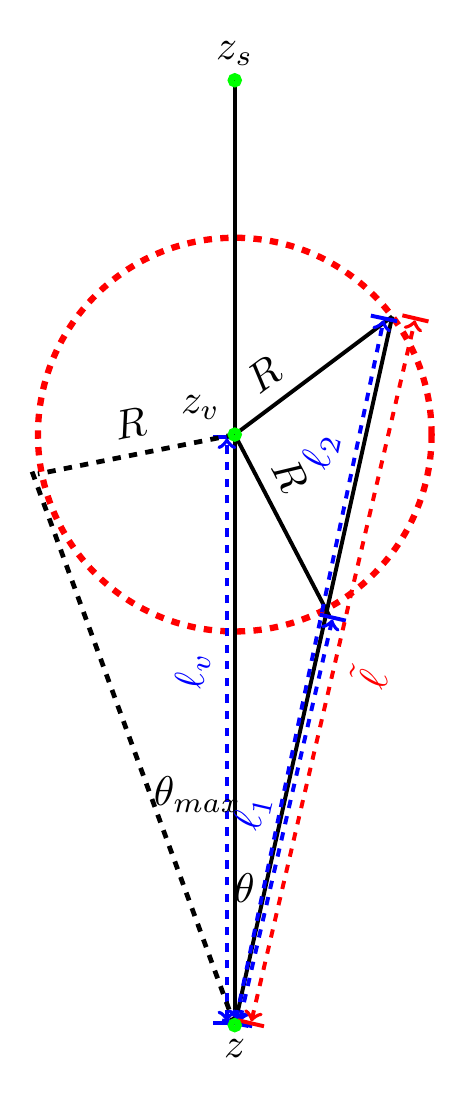
\begin{tikzpicture}[every node/.style={scale=1.5}] % Increase the scale for larger text

    \draw [line width=0.8mm, red,dashed] (0,7.5) circle (2.5cm);
   
    \draw [line width=0.5mm] (0,0) -- (0,12);
    \draw[|<->|] [line width=0.5mm, blue, dashed] (-.1,0) -- (-.1,7.5) node[pos=0.6, sloped, above] {$\ell_v$};
    \draw [line width=0.5mm] (0,7.5) -- (2,9) node[pos=0.3, sloped, above] {$R$};
    \draw[line width=0.5mm]  (0,7.5) -- (1.2,5.2) node[pos=0.3, sloped, above] {$R$};
    \draw [line width=0.5mm] (0,0) -- (2,9) node[pos=0.15, above] {$\theta~~$};
    \draw[|<->|] [line width=0.5mm, blue, dashed] (0.05,0) -- (1.25,5.2) node[pos=0.5, sloped, above] {$\ell_{1}$};
    \draw[|<->|] [line width=0.5mm, blue, dashed] (0.0,0) -- (1.9,9.0) node[pos=0.8, sloped, above] {$\ell_{2}$};
    \draw[|<->|] [line width=0.5mm, red, dashed] (0.2,0) -- (2.3,9.0) node[pos=0.5, sloped, below] {$\tilde{\ell} $};
    \draw [line width=0.6mm, dashed] (0,0) -- (-2.6,7.1) node[pos=0.35, above] {$ ~ ~ ~ ~ ~ \theta_{max}$};
    \draw [line width=0.6mm, dashed] (0,7.5) -- (-2.5,7.0) node[pos=0.5, sloped, above] {$R$};
    \node[below] at (0,0) {$z$};
    \node[above left] at (0,7.5) {$z_{v}$};
    \draw [line width=0.8mm, green] (0,0) circle (0.5mm);
    \draw [line width=0.8mm, green] (0,7.5) circle (0.5mm);
    \draw [line width=0.8mm, green] (0,12) circle (0.5mm);
    \node[above] at (0,12) {$z_{s}$};    
  \end{tikzpicture}

\end{document}